\chapter{Slaid persembahan}

\section{Membuat slaid \index{persembahan}persembahan dengan \latex{} beamer}
Kebiasaanya apabila kita mendengar \emph{presentation slides} maka yang terlintas di fikiran kita samada Microsoft(TM) PowerPoint ataupun OfficeOffice.org Impress.
Sebenarnya, \latex{} juga mempunyai pakej persembahannya yang dipanggil \mbox{"}beamer\mbox{"}.

Untuk pakej \index{beamer}beamer, kita perlu mengisytiharkan penggunaan pakej beamer, sama seperti sebelum ini:\\

\begin{Verbatim}[frame=single]
 \usepackage{beamer}
\end{Verbatim}

\subsection{Bingkai (\emph{frame})}
Di dalam beamer, setiap persembahan dipecahkan kepada beberapa bingkai atau di sini kita sebut sebagai frame. 
Cuba perhatikan kod berikut:


\begin{Verbatim}[frame=single]
 \begin{frame}
  
 \end{frame}
\end{Verbatim}

Dan sekarang tengok pula kod untum muka utama slaid kita:

\begin{Verbatim}[frame=single]
\documentclass[xcolor=dvipsnames,11pt]{beamer}
\usetheme{Luebeck} % ini untuk pilihan tema


\title[tutorial \LaTeX{}]{Pengenalan Kepada \LaTeX{}} 
% ini untuk tajuk di kaki slaid, pilihan saja

\author[Aiman]{Ahmad Abu Aiman }
% ini untuk tajuk di kaki slaid, plihan saja

\begin{document}
\begin{frame}

\title[Seminar \LaTeX{}, Segambut Dalam]{Pengenalan Kepada \LaTeX{}}
\author[Aiman]{Ahmad Abu Aiman }
\institute{
        Nama Institut,\\
        Malaysia\\
        }
\date{} 
% sekiranya tidak diisi dengan tarikh, tarikh 
%pada dokumen ini dikompil akan digunakan

\titlepage 
%ini untuk mengisytiharkan yang bingkai
% ini akan digunakan untuk muka depan


\begin{center}\texttt{email@email.com}\\
        \textrm{\tiny { Ditulis dengan \LaTeX{}}}
\end{center}


\end{frame}
\end{document}

\end{Verbatim}

\begin{minipage}{\textwidth}
Contoh output:
\begin{center}
\fbox{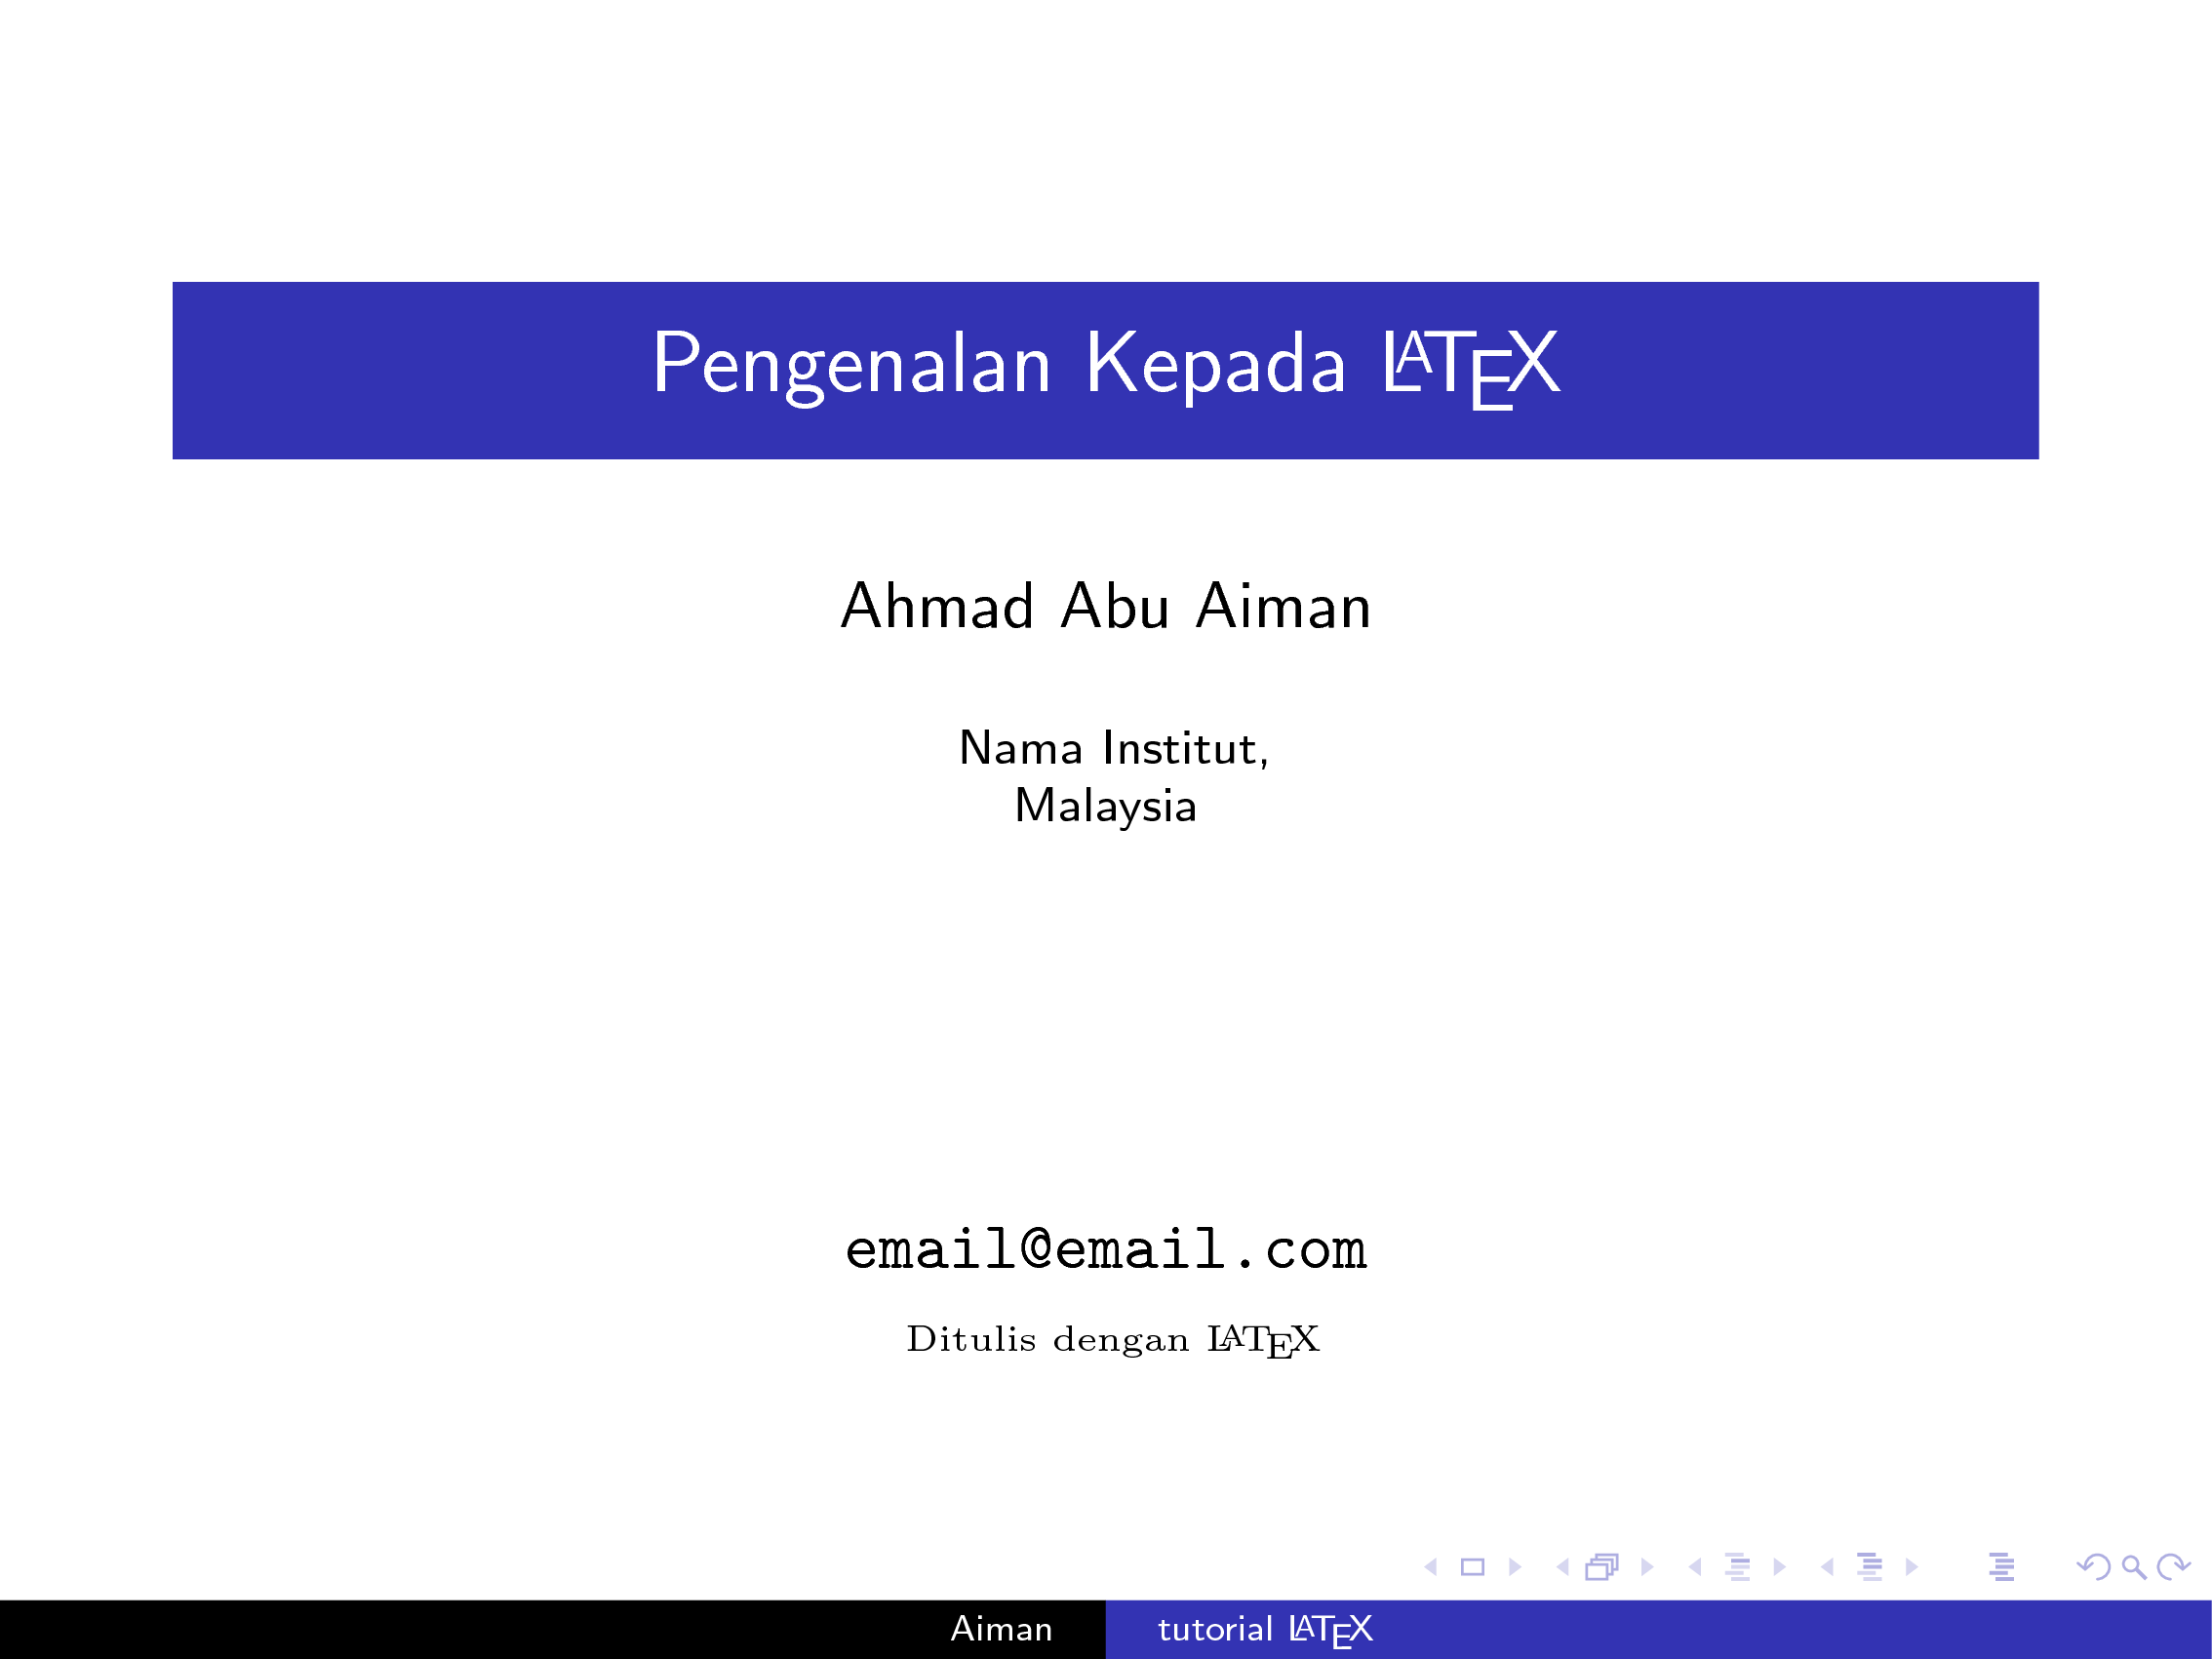
\includegraphics{beamer.png}}
\end{center}
\end{minipage}
